\def\title{اظهارنامه(مربوط به انتشار رساله/پایان نامه)}
\def\tashakor{\large{تشکر و قدردانی}}
\def\date{تاریخ \quad امضای دانشجو}
\newpage
\baselineskip=0.75cm‎‎‎‎

\begin{center}
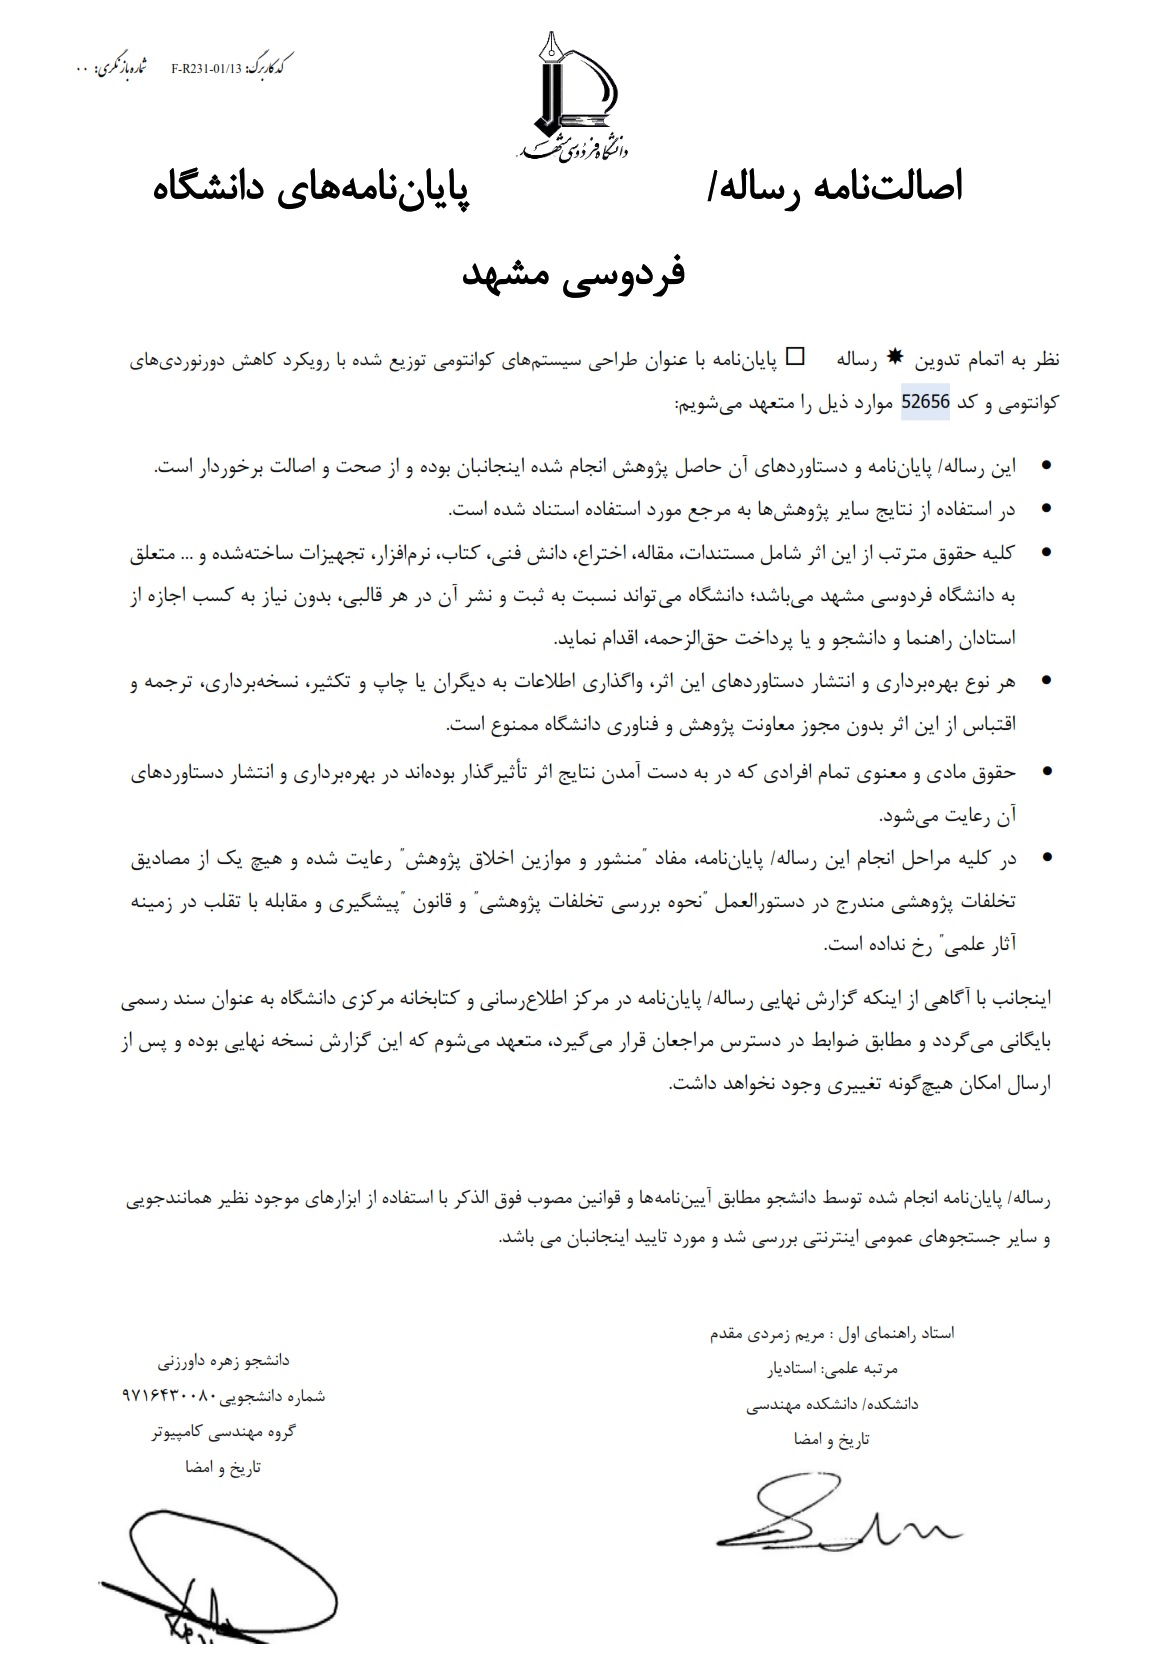
\includegraphics[scale=0.6]{esalat.jpg}\\
\end{center}
\newpage
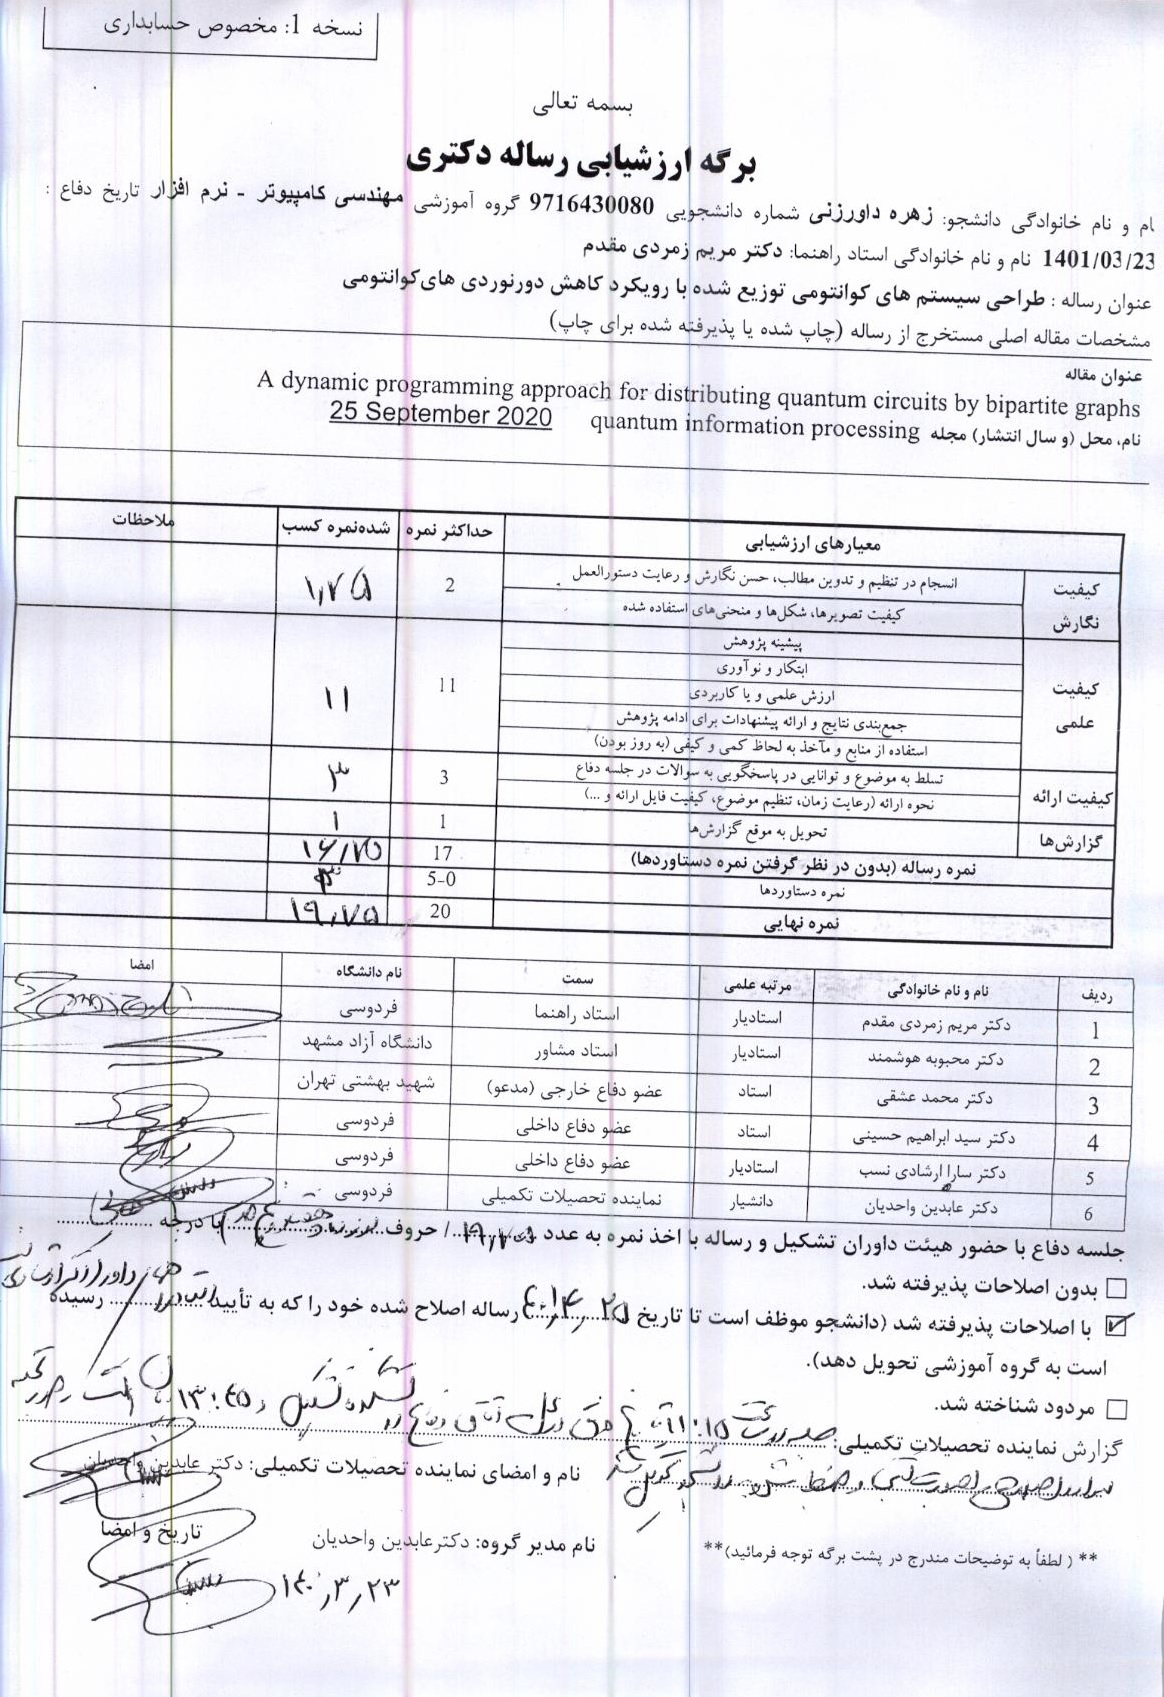
\includegraphics[scale=0.7]{arzesh.jpg}
\newpage
\KashidaOff
\begin{sols}

تقدیم به آنکه \\
\begin{center}
``تلاش مفهوم زندگی است'' 
\end{center}
\begin{flushleft}
را سرلوحه زندگی‌ام قرار داد.
\end{flushleft}

\end{sols}
\newpage
\begin{nazanint}
\begin{center}
\tashakor

منت خدای را عز و جل که طاعتش موجب قربت است و به شکر اندرش مزید نعمت.
\end{center}


در آغاز این رساله، بر خود می‌دانم از استاد بزرگوارم سرکار خانم دکتر مریم زمردی مقدم که با رهنمودهای ارزشمندشان همواره راهنما و چراغ راه من بوده‌اند، سپاس‌گزاری نمایم. حسن خلق، صبوری و همراهی این استاد گرانقدر همواره مایه‌ی آرامش و دلگرمی من در طول این دوره بوده است.

از سرکار خانم دکتر محبوبه هوشمند که با مشاوره‌های بسیار مفید و نکته‌های دلاویزشان راهگشای من در اتمام و اکمال این رساله بودند، تشکر نمایم.

همچنین، از سال‌ها زحمات و تلاش‌های بی‌دریغ کلیه اساتید محترم خویش در دانشگاه فردوسی مشهد که در تکوین دیدگاه من در دوره‌های کارشناسی، کارشناسی ارشد و دکتری نقش اساسی داشته اند، صمیمانه سپاس‌گزاری نمایم.

از پدر و مادر عزیزم، پشتیبان بی‌قید و شرط و همیشگی زندگی‌ام متشکرم.

از همسر مهربان و فرزند عزیزم که در این سال‌ها، پشتیبان، همراه و مشوق من بوده‌اند و این پژوهش بدون صبر و همراهی‌شان به سر انجام نمی‌رسید، سپاسگزارم. 
\end{nazanint}


\KashidaOn